\documentclass[12pt,a4paper]{article}
\usepackage[utf8]{inputenc}
\usepackage[english]{babel}
\usepackage[T1]{fontenc}
\usepackage{amsmath}
\usepackage{amsfonts}
\usepackage{amssymb}
\usepackage{graphicx}
\usepackage{verbatim}
\usepackage[left=2cm,right=2cm,top=2cm,bottom=2cm]{geometry}
\usepackage{siunitx}
\usepackage{placeins}
\usepackage{physics}
\author{Tim}
\usepackage{gensymb}
\usepackage{mathtools}
\usepackage{physics}
\begin{document}
\sisetup{separate-uncertainty = true}
	\setlength{\parindent}{0pt} 
	\begin{center}
		{\LARGE Exam}\\
		\begin{large}
			Computational Physics\\[0.4cm]
			Prof. Michielsen, Prof. Mazzarello\\[5.5cm]
			\Large\textbf{\textsl{Exercise 1: Quantum harmonic oscillator}}\\[5.5cm]
			\normalsize\textit{authored\\by}\\[0.4cm]
			\large\textbf{Moritz Berger (355244)\\moritz.berger@rwth-aachen.de}\\[2cm]
			\large{23.07.2019}
		\end{large}
	\end{center}
	\newpage
\section{Introduction}

In this exercise the behavior of a quantum harmonic oscillator is analyzed. It is described by a wave function in a quadratic potential
$$
V = \dfrac{\Omega^2}{2} x^2
$$
where $\Omega$ denotes the frequency of the oscillator. The equation of motion of this system is given by the one dimensional Schrödinger equation:
\begin{equation}
i \dfrac{\partial}{\partial t} \Phi(x,t) = \left(-\dfrac{1}{2}\dfrac{\partial^2}{\partial x^2} + \dfrac{\Omega^2}{2} x^2\right) \Phi(x,t) = H \Phi(x,t)
\end{equation}
with all variables being dimensionless ($\hbar = m = 1$).\\
The goal is to simulate the time evolution of the wave function for different starting functions and to compute the average and variance of this function over time.
\section{Simulation Model and Method}

The simulated area is a one dimensional grid ranging from $-15\leq x\leq 15$ that is split into $L=1001$ equally spaced points. This results in a step width of $\Delta = 0.03$. The initial wave function is described by a Gaussian function:
\begin{equation}
\Phi_0(x,t=0) = \dfrac{1}{\pi \sigma^2} e^{-(x-x_0)^2/2\sigma^2}
\end{equation}
5 different combinations of the oscillator frequency $\Omega$, $\sigma$ and $x_0$ are simulated. \\
\\
The Schrödinger equation is solved by using a second order product formula approach. For this the spacial derivative in the Hamiltonian $H$ is approximated by a 3 point formula:
\begin{equation}
\dfrac{\partial^2}{\partial x^2} \Phi(x,t) = \dfrac{\Phi(x+\Delta,t) - 2\Phi(x,t) + \Phi(x-\Delta,t)}{\Delta^2}
\end{equation}

The Schrödinger equation can then be written as a matrix-vector equation where the vector elements correspond to the spacial positions and $H$ is expressed as:
$$ H= \Delta^{-2} \left(\begin{matrix}1+\Delta^2V_1&\frac{-1}{2}&0&0\\\frac{-1}{2}&1+\Delta^2V_2&\frac{-1}{2}&0\\&&...&\\0&0&\frac{-1}{2}&1+\Delta^2V_L\end{matrix}\right) $$

The time evolution of the wave function after a time step $\tau$ is given by
\begin{equation}
\Phi(x,t+\tau) = e^{-i\tau H} \Phi(x,t)
\end{equation}
For this exercise a time step of $\tau = 0.00025$ and a number of steps of $m = 40000$ is used, resulting in a total simulation time of $t = 10$.\\
Calculation of the time evolution operator $U = e^{-i\tau H}$ can be problematic if $H$ cannot be brought to diagonal form. In the product formula approach this is circumvented by splitting $H$ into different matrices:
\begin{equation}
H = V + K_1 + K_2
\end{equation}
The matrix V consists only out of the diagonal elements of H and is therefore already diagonal. $K_1$ and $K_2$ contain the off-diagonal elements. They are constructed in a way so that the matrices $e^{-i\tau K_{1,2}/2}$ can be described as block diagonal matrices with a 2x2 matrix as block:
$$ \left(\begin{matrix}cos(a)&isin(a)\\isin(a)&cos(a)\end{matrix}\right) $$
with $a = \tau/4\Delta^2$. These matrices are unitary, which allows the calculation of $U$:
\begin{equation}
U = e^{-i\tau K_1/2} e^{-i\tau K_2/2} e^{-i\tau V} e^{-i\tau K_2/2} e^{-i\tau K_1/2} 
\end{equation}

With this the wave function for each time step is calculated from the result of the previous time step. The probability distribution is then calculated in the following way:
$$ P(x,t) = \int_{a}^{b} |\Phi(x,t)|^2 dx = |\Phi(x,t)|^2 \Delta$$
The multiplication with $\Delta$ is necessary in order to achieve correct normalization, because we compute the discrete function. This factor would vanish for the continuous function. The probability is calculated for $t = 0,2,4,...,10$.\\
\\
The expectation values
$$ \expval{x(t)} = \int_{-\infty}^{\infty} x|\Phi(x,t)|^2 dx$$
and
$$ \expval{x^2(t)} = \int_{-\infty}^{\infty} x^2|\Phi(x,t)|^2 dx$$
are calculated by a numerical integration over the whole simulation area following the Simpson rule. The amplitude of the wave function outside of the area is assumed to be small and can be neglected. This calculation is done every 200 time steps, which equates to a calculation in steps of $0.05$.

\section{Analytical Results}
The analytical solution for the average position and variance can be derived using the Ehrenfest theorem. Using it we get the following equation for $\expval{x}$:
\begin{equation}
\dfrac{d^2}{dt^2} \expval{x} = \Omega^2 \expval{x}
\end{equation}
which is also the equation of motion for a classical oscillator. The solution using the initial wave function is:
\begin{equation}
\expval{x(t)} = x_0 \cos(\Omega t)
\end{equation}
For $\expval{x^2}$ we get the differential equation:
\begin{equation}
\dfrac{d^2}{dt^2} \expval{x^2} = 4\expval{E} - 4\Omega^2 \expval{x^2}
\label{eq:2x}
\end{equation}
with the expectation value of the energy
\begin{equation}
\expval{E} = \dfrac{1}{2}\Omega^2 \left(\dfrac{\sigma^2}{2} + x_0^2\right) + \dfrac{1}{4\sigma^2}
\end{equation}
Equation \ref{eq:2x} can be solved for our initial wave function resulting in:
\begin{equation}
\expval{x^2(t)} = \dfrac{\expval{E}}{\Omega^2} + \left(\dfrac{\sigma^2}{2} + x_0^2 - \dfrac{\expval{E}}{\Omega^2}\right) \cos(2\Omega t)
\end{equation}
From this we can calculate the Variance. In summary the analytical solutions are:
\begin{equation}
\expval{x(t)} = x_0 \cos(\Omega t)
\label{eq:xexp}
\end{equation}
\begin{equation}
\expval{x^2(t)} - \expval{x(t)}^2 = \dfrac{1}{4} \sigma^2 + \dfrac{1}{4 \Omega^2 \sigma^2} + \dfrac{1}{4}\left(\sigma^2 - \dfrac{1}{\Omega^2 \sigma^2}\right) \cos(2\Omega t)
\label{eq:2xexp}
\end{equation}

\section{Results}
The probability distributions of 5 simulations with different parameters are shown in figure \ref{fig:prob}. The average position and the variance of the wave function are plotted in figure \ref{fig:av}. The average position seems to oscillate with a amplitude of $x_0$ and a period of $\Omega$. The variance of the wave function also oscillates based on the values of $\Omega$ and $\sigma$. With $\Omega = \sigma = 1$ the variance is constant and the probability distribution keeps the same form. However when using different values it starts oscillating, changing the height of the peak. The oscillation frequency of the variance is about two times as large as the frequency of the average position.

\begin{figure}
\centering
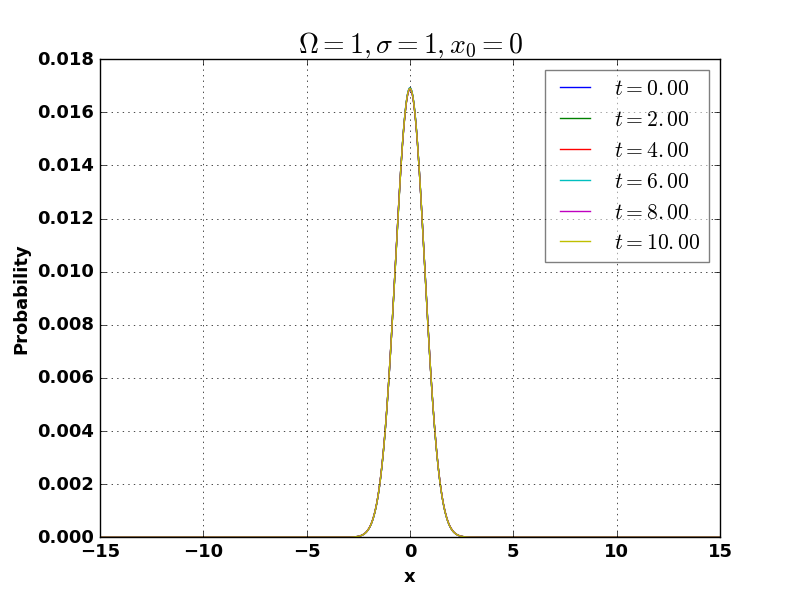
\includegraphics[scale=0.4]{Bilder/110.png}
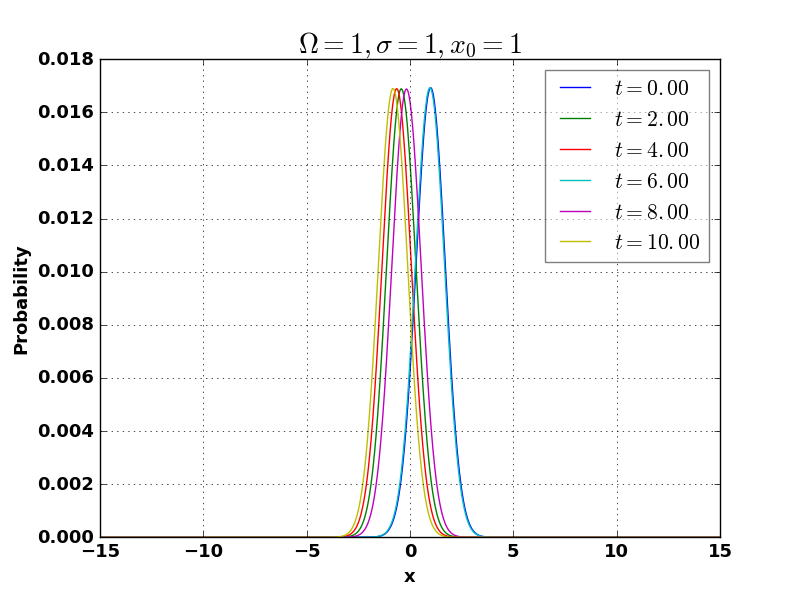
\includegraphics[scale=0.4]{Bilder/111.png}
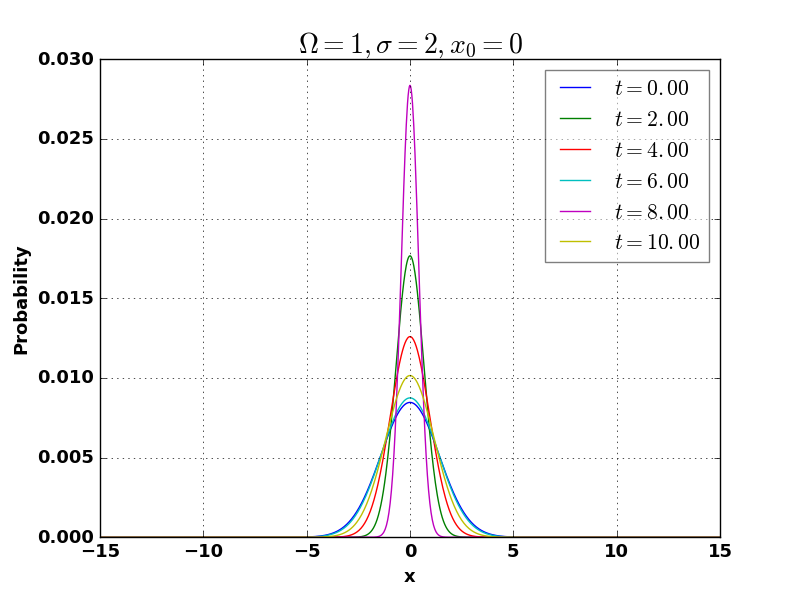
\includegraphics[scale=0.4]{Bilder/120.png}
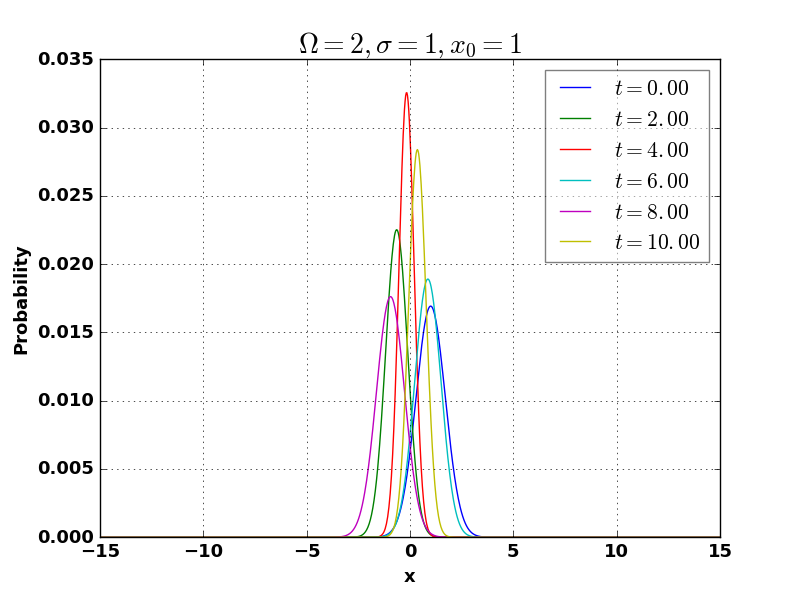
\includegraphics[scale=0.4]{Bilder/211.png}
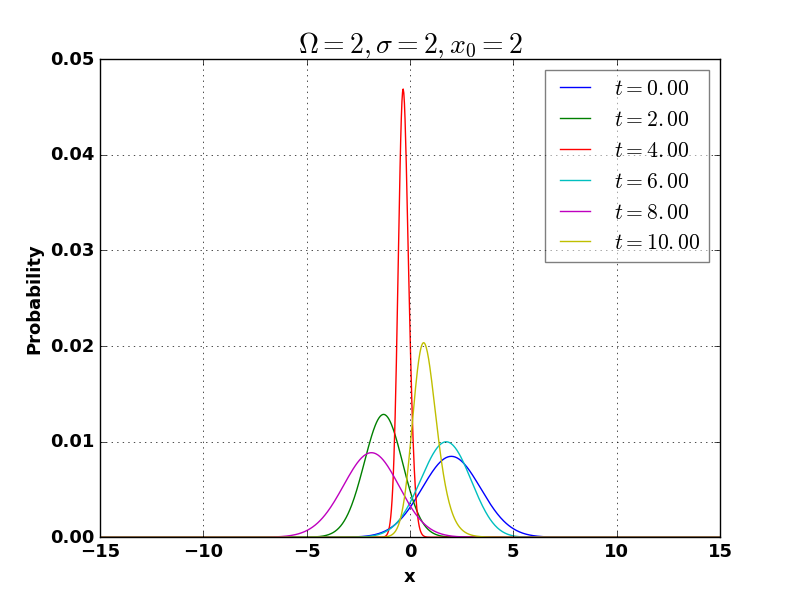
\includegraphics[scale=0.4]{Bilder/222.png}
\caption{Probability distribution of the wave function for all simulated combinations of parameters taken after $t = 0,2,4,...,10$.}
\label{fig:prob}
\end{figure}

\begin{figure}
\centering
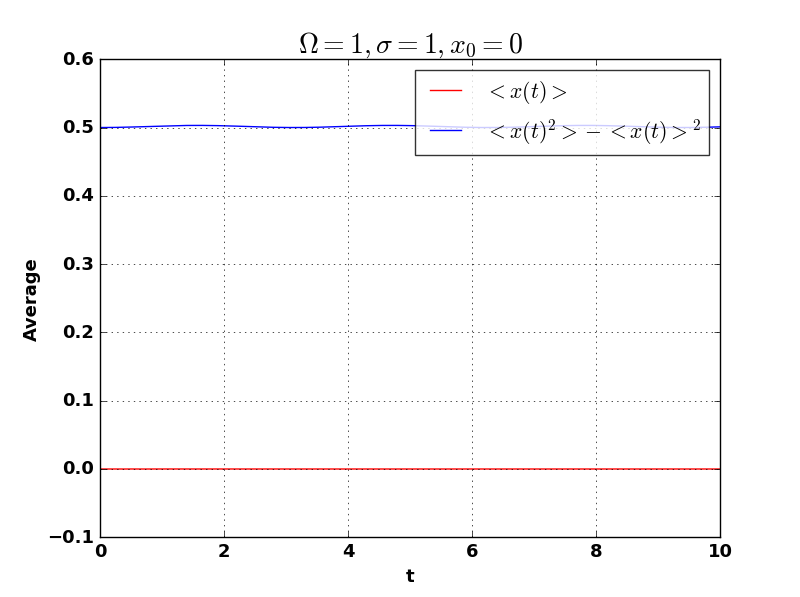
\includegraphics[scale=0.4]{Bilder/110_av.png}
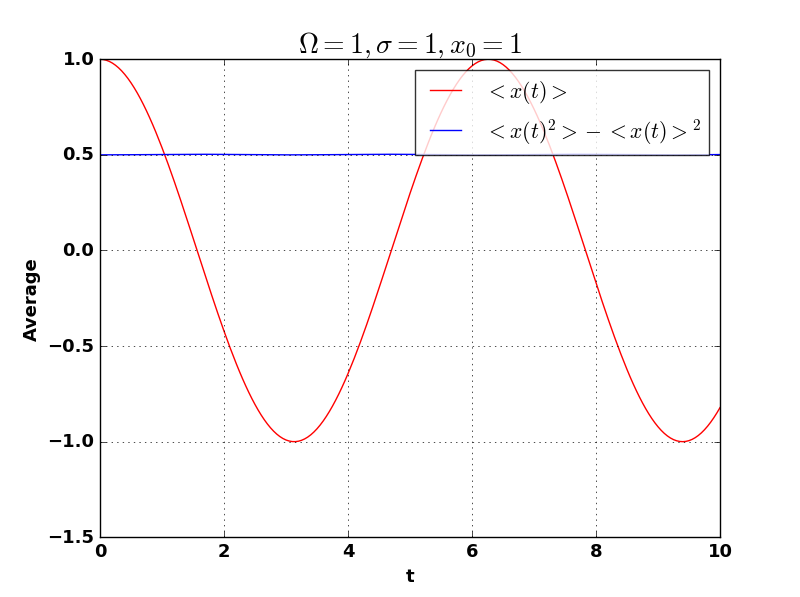
\includegraphics[scale=0.4]{Bilder/111_av.png}
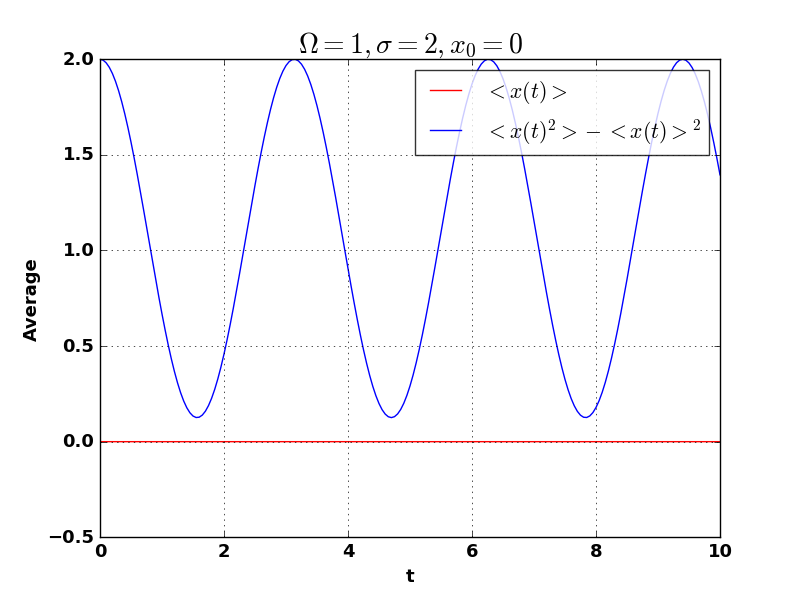
\includegraphics[scale=0.4]{Bilder/120_av.png}
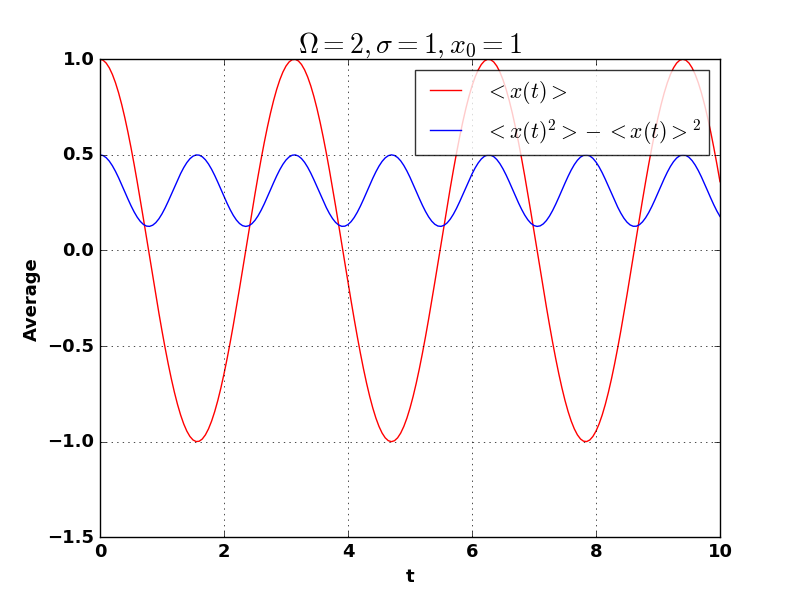
\includegraphics[scale=0.4]{Bilder/211_av.png}
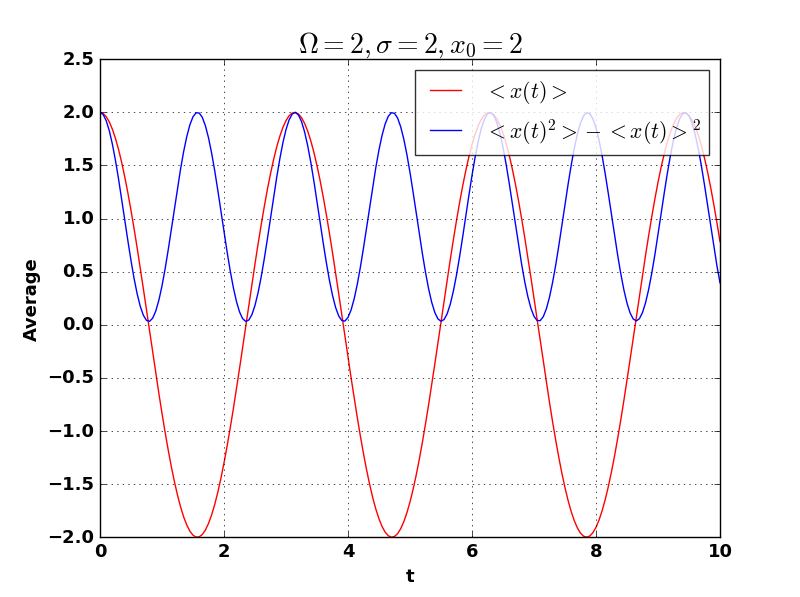
\includegraphics[scale=0.4]{Bilder/222_av.png}
\caption{Position and variance of the wave function plotted against the time.}
\label{fig:av}
\end{figure}


\section{Discussion}
The quantum harmonic oscillator behaves similar to a classical harmonic oscillator. The numerical solution for $\expval{x(t)}$ is in agreement with the analytical solution \ref{eq:xexp}, which is the same as the motion of a classical harmonic oscillator. The Variance $\expval{x^2(t)} - \expval{x(t)}^2$ also shows an oscillatory behavior, which is in agreement with the analytical solution \ref{eq:2xexp}. In figure \ref{fig:dif} the difference between the numerical and analytical solutions is shown. Both position and variance show an oscillating error. This error is introduced by the discretization and approximation of the spacial derivative. The error grows over time because the result for one time step is dependent on the previous one, which means that it carries over to the next time step.

\begin{figure}
\centering
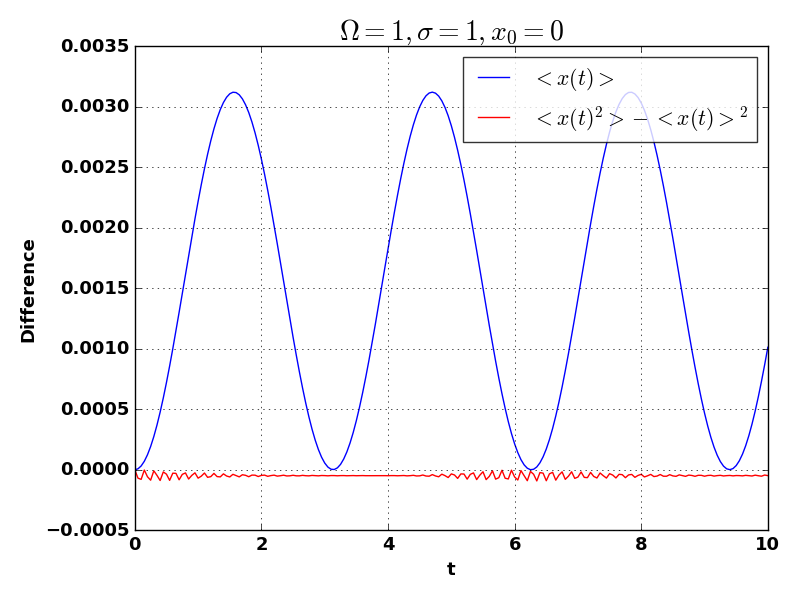
\includegraphics[scale=0.4]{Bilder/110_dif.png}
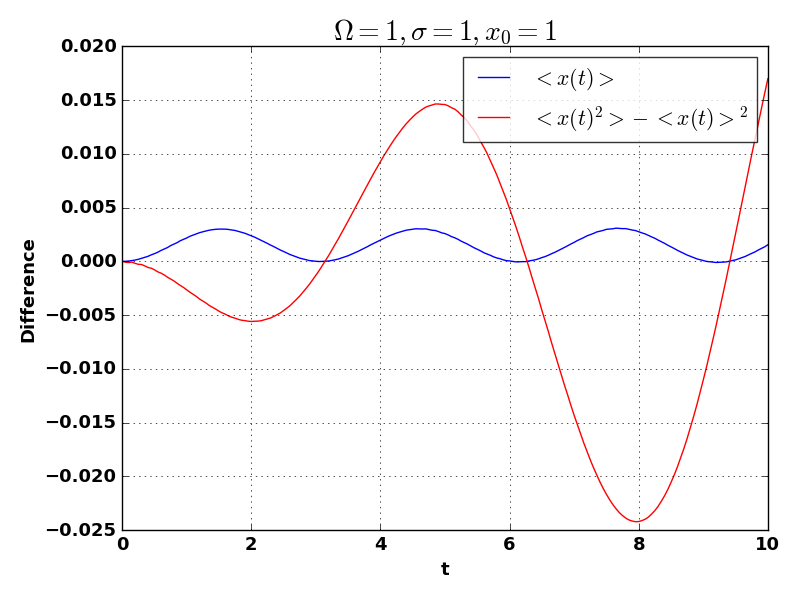
\includegraphics[scale=0.4]{Bilder/111_dif.png}
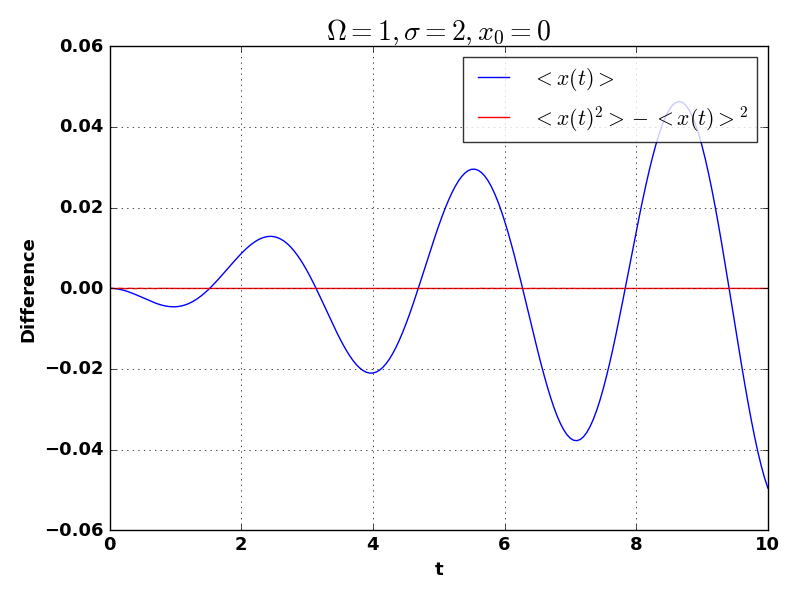
\includegraphics[scale=0.4]{Bilder/120_dif.png}
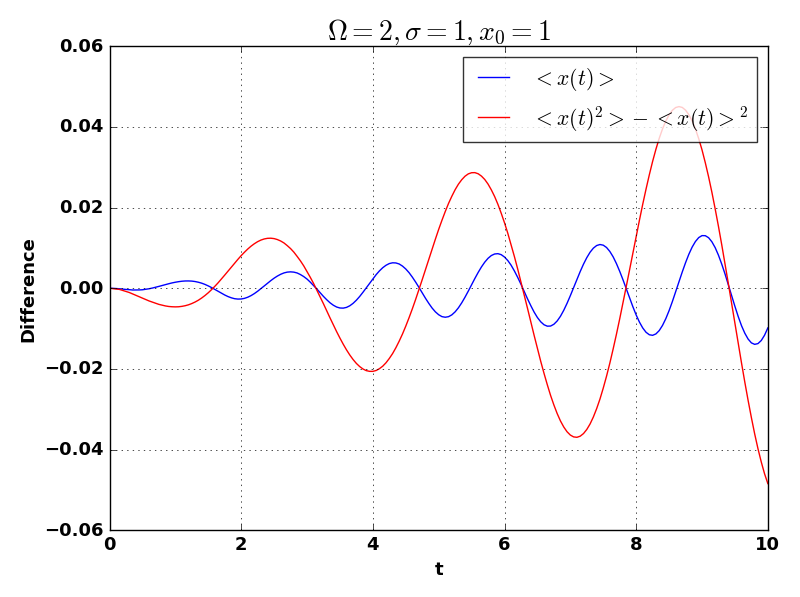
\includegraphics[scale=0.4]{Bilder/211_dif.png}
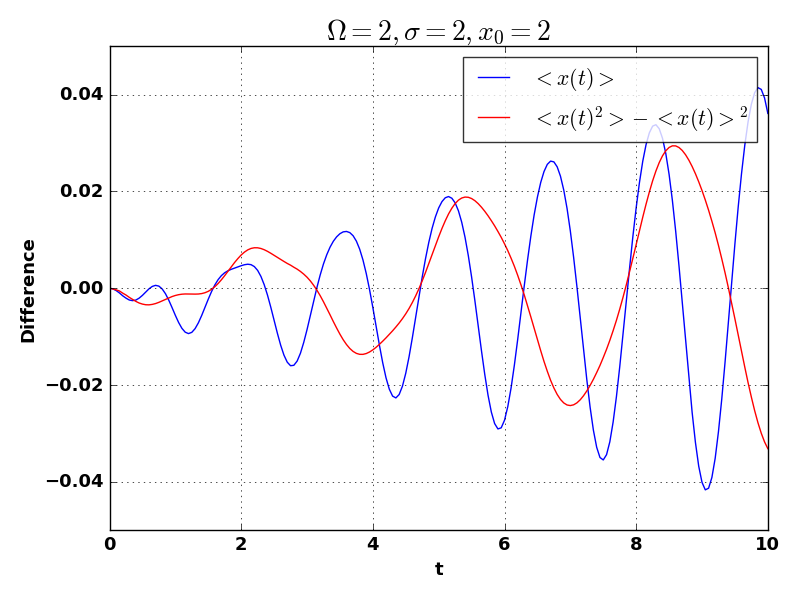
\includegraphics[scale=0.4]{Bilder/222_dif.png}
\caption{Difference between the numerical and analytical solution for the position and variance.}
\label{fig:dif}
\end{figure}

\end{document}



\